\documentclass{article}
\usepackage{amsmath,amsthm,mathrsfs,amssymb,graphicx,hyperref,url}
\usepackage{geometry}
\title{PHYS 215C In-Class Notes}
\author{Bill Wolf, Keith Fratus}
\date{Spring 2011}
\begin{document}
\maketitle \newpage{}
\tableofcontents
 \newpage{}
		\textit{March 28, 2011}	
	\section{Scattering}
		\subsection{Suggested References}
		\begin{itemize}
			\item Sakurai Ch. 6
			\item Shankar Ch. 19
			\item Merzbacher Ch. 11
		\end{itemize}
		\subsection{Basic Setup}
		The basic idea in scattering theory is a particle being scattered into a target (particle into target). Other models model two particles moving towards each other and scattering off each other (particle into particle).
		\subsubsection{Applications}
		Particle into particle scattering is very prevalent in high energy physics studies (particle accelerators), with traditional subatomic particles like electrons, neutrons, and protons.\\
		
		\noindent Target scattering is used to model particle-particle interactions (particle physics), atoms and ions (atomic/nuclear physics), and interactions within a solid or liquid (condensed matter physics).
		
		\subsection{Scattering Approach to ${e^-}$ Transport in solids}
		\subsubsection{Setup}
		In this theory we talk about the conduction of electrons in a metal or doped semiconductor. The canonical experiment is a battery providing a potential difference across the material of interest. The conductance, $G=I/V=1/R$, is what is of interest. There are impurities in the metal or semiconductor that cause scattering of the electrons that are moving under the influence of the potential difference.
		\subsubsection{Rolf Landauer's Theory (Landauer Transport Theory)}
		\paragraph{Toy Model} Consider a one-dimensional scattering potential that is a finite potential barrier between $x=a$ and $x=-a$ with incident electrons coming from the left with average energy $E$. (This is actually very relevant in a gated two-dimensional electron gas, where the low energies only allow one mode on the surface dimension.) The theory of this problem is well understood in terms of transmission and reflection coefficients (see the appendix in Sakurai). We will look at the \emph{steady state} system.\\
		
		\noindent First divide the region up into three regions. Region I is $-\infty<x<-1$, region II is $-a<x<a$, and region III is $a<x<\infty$. This gives rise to three wave functions of interest.
		\begin{align*}
			\psi_{\mathrm{I}}&=A_{\mathrm{in}}e^{ikx}+A_{\mathrm{out}}e^{-ikx}\\
			\psi_{\mathrm{II}}&=C_1e^{ik'x}+C_2e^{-ik'x}\\
			\psi_{\mathrm{III}}&=B_{\mathrm{out}}e^{9kx}+B_{\mathrm{in}}e^{-ikx}
		\end{align*}
		where $$k=\frac{1}{\hbar}\sqrt{2mE}\qquad k'=\frac{1}{\hbar}\sqrt{2m(E-V)}$$
Normally we would solve for these wave functions by matching $\psi$ and $\psi'$ at the boundaries to relate $A,B,$ and $C$. We can represent the solution via a transfer matrix:
$$\left(\begin{array}{c}B_{\mathrm{out}} \\B_{\mathrm{in}}\end{array}\right)=\left(\begin{array}{cc}M_{11} & M_{12} \\M_{21} & M_{22}\end{array}\right)\left(\begin{array}{c}A_{\mathrm{in}} \\A_{\mathrm{out}}\end{array}\right)$$


% I need to get the figure file from Bill - Keith
% Done! 4/2/2011 - Bill
\begin{figure}[h]
	\centering
	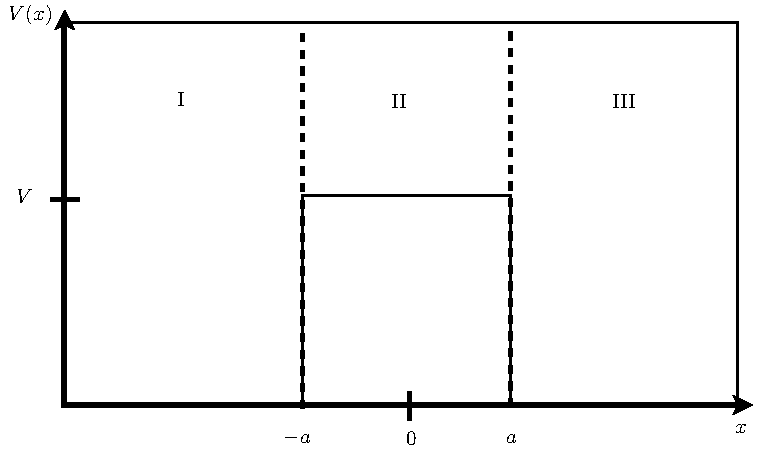
\includegraphics{Fig_1.pdf}
	\caption{1-D Scattering Potential}
\end{figure}
Alternatively, we may use the less clear $S$-matrix:
			$$\left(\begin{array}{c}A_{\mathrm{out}} \\B_{\mathrm{out}}\end{array}\right)=\left(\begin{array}{cc}S_{11} & S_{12} \\S_{21} & S_{22}\end{array}\right)\left(\begin{array}{c}A_{\mathrm{in}} \\B_{\mathrm{in}}\end{array}\right)$$
			The system obeys an equation of continuity (probability conservation):
			$$\partial_t\left|\psi\right|^2+\partial_xJ=0$$
			where
			$$J=\frac{\hbar}{m}\mathrm{Im}\left(\psi^*\partial_x\psi\right)$$
			The currents in regions I and III gives
			\begin{align*}
				J_{\mathrm{I}}&=\frac{\hbar k}{m}\left[\left|A_{\mathrm{in}}\right|^2-\left|A_{\mathrm{out}}\right|^2\right]\\
				J_{\mathrm{III}}&=\frac{\hbar k}{m}\left[\left|B_{\mathrm{out}}\right|^2-\left|B_{\mathrm{in}}\right|^2\right]
			\end{align*}
			The equation of continuity then tells us that
			$$\left|A_{\mathrm{out}}\right|^2+\left|B_{\mathrm{out}}\right|^2=\left|A_{\mathrm{in}}\right|^2+\left|B_{\mathrm{in}}\right|^2$$
			$$\left(\begin{array}{cc}A_{\mathrm{out}}^* & B_{\mathrm{out}}^*\end{array}\right)\left(\begin{array}{c}A_{\mathrm{out}} \\A_{\mathrm{out}}\end{array}\right)=\left(\begin{array}{cc}A_{\mathrm{in}}^* & B_{\mathrm{in}}^*\end{array}\right)S^\dagger S\left(\begin{array}{c}A_{\mathrm{in}} \\B_{\mathrm{in}}\end{array}\right)$$
			For scattering states, we let $B_{\mathrm{in}}=0$, that is, particles are \emph{only} incident from the left. Then we have
			$$\psi_k(x)=\begin{cases} A_{\mathrm{in}}e^{ikx}+A_{\mathrm{out}}e^{-ikx} & x<-a\\
			B_{\mathrm{out}}e^{ikx} &x>a \end{cases}$$
			and we have
			\begin{align*}
				B_{\mathrm{out}}&=S_{21}A_{\mathrm{in}}\\
				A_{\mathrm{out}}&=S_{11}A_{\mathrm{in}}
			\end{align*}
			We define transmission and reflection coefficients
			\begin{align*}
			T&\equiv \frac{\left|B_{\mathrm{out}}\right|^2}{\left|A_{\mathrm{in}}\right|^2}=\left|S_{21}\right|^2\\
			R&\equiv \frac{\left|A_{\mathrm{out}}\right|^2}{\left|A_{\mathrm{in}}\right|^2}=\left|S_{11}\right|^2\\
			\end{align*}
			\paragraph{Landauer Formula}
			$$G=\frac{I}{V}\Rightarrow G=\frac{e^2}{h}T$$
			where $e^2/h$ is the quantum of conductance.\\
			
			\noindent \textit{March 30, 2011}
			\subsubsection*{Derivation of the Landauer Formula}
			Suppose we send in a wave with wave number $k$ and energy $E=\hbar^2k^2/2m$ from the left. As expected, we would get a portion of the wave to be reflected (proportional to $S_{11}$) the remainder to to be transmitted (proportional to $S_{21}$).	\\		
			
			\noindent The Scattering State is then given by
			$$\psi_{1}^k(x)=\begin{cases} \frac{e^{i\phi_1 k}}{\sqrt{2\pi}}\left(e^{ikx}+S_{11}e^{-ikx}\right) & x<-a\\
			\frac{e^{\phi_1k}}{\sqrt{2\pi}}S_{21}e^{ikx} & x>a \end{cases}$$
			$$\psi_2^k(x)=\begin{cases} \frac{e^{i\phi_2 k}}{\sqrt{2\pi}}\left(e^{ikx}+S_{22}e^{ikx}\right) & x>a\\
			\frac{e^{\phi_2k}}{\sqrt{2\pi}}S_{12}e^{-ikx} & x<-a \end{cases}$$
			With this, we are ready to\ldots\\
			
			\noindent For $T=0$, we have incident electrons up to chemical potential $\mu$. On different leads on a quantum wire, we generally have two different chemical potentials, which causes a net transport of electrons. Suppose on the left we have $\mu_1$ and on the right we have $\mu_2$ with $\mu_1<\mu_2$, which causes an electrical net current from left to right. Our goal is to study this current in terms of the $S$-matrix.
			\paragraph{Fermi Wave Number} We define the Fermi Wave Number by
			$$k_F=\frac{1}{\hbar}\sqrt{2m\mu}$$
			The probability current for $e^{-1}$ at $k$ is given by
			$$J_j^k=\frac{\hbar}{m}\mathrm{Im}\left[{\psi_j^k}^*(x)\partial_x \psi_j^k(x)\right]$$
			The electrical current is then
			$$\left.I\right|_{x>a}=e J_j^k=e\frac{\hbar}{m}\left[\int_0^{k_{F_1}}dk\,\frac{k}{2\pi}\left|S_{21}\right|^2+\int_{0}^{k_{F_2}}dk\frac{k}{2\pi}\left(-1+\left|S_{22}\right|^2\right)\right]$$
			Then the transmission probability if $T_k\equiv\left|S_{21}\right|^2$, which gives the current to be
			$$I=\frac{e}{2\pi}\int_{k_{F_2}}^{k_{F_1}}dk\,\left(\frac{\hbar k}{m}\right)T_k=\frac{3}{2\pi\hbar}\int_{\mu_2}^{\mu_1} dE\,T(E)$$
			Where we have used $E=\hbar2k^2/2m$ and $dE=(\hbar^2k/m)\,dk$. We may relate the two chemical potentials to the electric voltage via
			$$\mu_1=\mu_2+eV$$
			\paragraph{Linear Response}
			The conductance is given by 
			$$G=\lim_{V\to0} \frac{I}{V}$$
			Then the electric current can be rewritten as
			$$I=\frac{e}{2\pi\hbar}\int_{\mu_2}^{\mu_2+eV}dE\,T(e)=\frac{e^2}{h}T(\mu)V$$
			and then the conductance in this linear response limit is
			$$G=\frac{I}{V}=\frac{e^2}{h}T(\mu)=\frac{e^2}{h}T(E_F)$$
			\subsubsection{Some Comments}
			\begin{enumerate}
				\item Suppose we have a perfect wire with \emph{no} backscattering. That is, $T=1$. Then we have $R=\frac{1}{G}=0$. This would of course be superconductivity.
				\item This theory can be generalized to multichannel wires with many leads. The resulting conductance for $N$ leads is then
				$$G=\frac{e^2}{h}2N$$
				where the factor of 2 comes from electron spin degeneracy.
				\item This theory has been validated by experiment with a quantum wire circuit setup that revealed a stair-step plot of conductance as a function of input voltage.
				\item We have ignored the fact that the electrons interact and experience interactions off of one another (calculations effectively carried out at zero temperature). As a result, these resistances do not necessarily add in series.
			\end{enumerate}
			\subsection{Inelastic Scattering}
			In the field of inelastic scattering, we typically consider the situation of a particle scattering off of a quantum mechanical system. This system could be a liquid, a solid, a nuclei\ldots anything, really. The inelastic condition implies that the act of scattering transfers energy between the particle and the target. 
			
			\subsubsection{Setup and Notation} To ease the theory, we will suppose that the ``target'' will be composed of particles with position operators $\mathbf{R}_i$ and momentum operators $\mathbf{P}_i$. The incident particle will have position operator $\mathbf{R}$ and $\mathbf{P}$. The Hamiltonian of the system will be
			
			%%%%%%%%%
			$$\hat{\mathscr{H}}=\frac{\mathbf{P}^2}{2m}+\hat{H}+V$$
			%%%%%%%%%
			
			Where the first term is the kinetic energy of the particle, the non-script Hamiltonian is the internal energy of the target (kinetic plus potential), and the term V is the interaction potential. To simplify the system, we shall assume that the interaction potential takes on the form
			
			
			$$V=\sum_{i=1}^N V(\mathbf{R}-\mathbf{R}_i)$$
			
			
			\paragraph{Density Operator} It becomes useful to define a density operator for the target. It is
			
			
			$$\rho(\mathbf{r})=\sum_{i=1}^N \delta^3(\mathbf{r}-\mathbf{R}_i)$$
			
			
			where $\mathbf{r}$ is simply a c-number position coordinate (multiplied by identity). We will use the Fourier transform of this operator,
			
			
			$$\rho(\mathbf{q})=\int d^3\mathbf{r}\,e^{-i\mathbf{q}\cdot\mathbf{r}}\rho(\mathbf{r})=\sum_{i=1}^Ne^{-i\mathbf{q}\cdot\mathbf{R}_i}$$
			
			
			\paragraph{Rewriting the Interaction Potential} This density operator can help us rewrite the potential into a more useful form:
			
			%%%%%%%%%%%%%%%%%%%%%%%%%%%%%%%%%%%%%%%%%%%%%%%%%%%%%%%%%%%%%%%%%%%%%%%
			\begin{equation} \label{eq:pot-dens}
			V=\sum_{i=1}^N \int\frac{d^3\mathbf{q}}{(2\pi)^3}V(\mathbf{q})e^{i\mathbf{q}\cdot(\mathbf{R}-\mathbf{R}_i)}=\int\frac{d^3\mathbf{q}}{(2\pi)^3}V(\mathbf{q}) \rho(\mathbf{q})e^{i\mathbf{q}\cdot\mathbf{R}}
			\end{equation}
			%%%%%%%%%%%%%%%%%%%%%%%%%%%%%%%%%%%%%%%%%%%%%%%%%%%%%%%%%%%%%%%%%%%%%%%
			
			which is just the definition of the Fourier Transform of the interaction potential in the first line, and then a re-expression in terms of the density operator in the second line.
			
			\subsubsection{Modeling Scattering}
			
			
			\paragraph{Fermi's Golden Rule} Suppose we start with an initial state $\left|\mathbf{k};\,E_i,\alpha\right>$, where \textbf{k} is the wavevector of the incoming particle, $E_{i}$ is the initial internal energy of the target and $\alpha$ indexes the particular state with energy $E$ (since there may be degeneracy). If we end with a final state $\left|\mathbf{k}';\,E_f,\beta\right>$, then Fermi's Golden Rule tells us
			
			
			$$\Gamma_{i\to f}=\frac{2\pi}{\hbar}\left|\left<\mathbf{k}';\,E_f,\beta\right|V\left|\mathbf{k};\,E_i,\alpha\right>\right|^2\delta(E_f+\epsilon_{k'}-E_i-\epsilon_k)$$
			
			
			Where the delta function maintains energy conservation (fuck you Bill). For brevity, we'll denote the matrix element as $V_{fi}$. In terms of the interaction potential, this matrix element is then, using equation \ref{eq:pot-dens},
			
			%%%%%%%%%%%%%%%%%%%%%%%%%%%%%%%%%%%%%%%%%%%%%%%%%%%%%%%%%%%%%%%%%%%%%%%
			\begin{equation} \label{eq:matrix}
			V_{fi}=\int\frac{d^3\mathbf{q}}{(2\pi)^3}V(\mathbf{q})\left<\mathbf{k}';\,E_f\beta\left|\rho(\mathbf{q})e^{i\mathbf{q}\cdot \mathbf{R}}\right|\mathbf{k};\,E_i\alpha\right>
			\end{equation}
			%%%%%%%%%%%%%%%%%%%%%%%%%%%%%%%%%%%%%%%%%%%%%%%%%%%%%%%%%%%%%%%%%%%%%%%
			
			We now make use of the fact that the momentum and position operators are conjugate operators:
		
			$$e^{ia\hat{p}/\hbar}\left|x\right>=\left|x+a\right>$$
			
			$$e^{iq\hat{x}}\left|k\right>=\left|k+q\right>$$
			
			So now we have
			
			$$e^{i\mathbf{q}\cdot\mathbf{R}}\left|\mathbf{k}\right>=\left|\mathbf{k}+\mathbf{q}\right>$$
			
			Now, the state ket we have written is really a direct product,
			
			%%%%%%%%%%%%%%%%%%%%%%%%%%%%%%%%%%%%%%%%%%%%%%%%%%%%%%%%%%%%%%%%%%%%%%%
			\begin{equation} \label{eq:dir-prod}
			\left|\mathbf{k};\,E_i,\alpha\right> = \left|\mathbf{k}\right> \otimes \left|E_i,\alpha\right>.
			\end{equation}
			%%%%%%%%%%%%%%%%%%%%%%%%%%%%%%%%%%%%%%%%%%%%%%%%%%%%%%%%%%%%%%%%%%%%%%%
			
			Since \textbf{R} only acts on the portion of the direct product pertaining to the incoming particle, and $\rho$(\textbf{q}) only acts on the portion of the direct product pertaining to the target, we can write,
			
			%%%%%%%%%%%%%%%%%%%%%%%%%%%%%%%%%%%%%%%%%%%%%%%%%%%%%%%%%%%%%%%%%%%%%%%
			\begin{equation} \label{eq:inner1}
			\left<\mathbf{k}';\,E_f,\beta\left| \rho(\mathbf{q}) e^{i\mathbf{q}\cdot\mathbf{R}}\right|\mathbf{k};\,E_i,\alpha\right> = \left<E_f,\beta\left| \rho(\mathbf{q}) \right|E_i,\alpha\right> \left<\mathbf{k}'\right|e^{i\mathbf{q}\cdot\mathbf{R}}\left.|\mathbf{k}\right>
			\end{equation}
			%%%%%%%%%%%%%%%%%%%%%%%%%%%%%%%%%%%%%%%%%%%%%%%%%%%%%%%%%%%%%%%%%%%%%%%
			
			%%%%%%%%%%%%%%%%%%%%%%%%%%%%%%%%%%%%%%%%%%%%%%%%%%%%%%%%%%%%%%%%%%%%%%%
			\begin{equation} \label{eq:inner2}
			 = \left<E_f,\beta\left| \rho(\mathbf{q}) \right|E_i,\alpha\right>  \left<\mathbf{k}'\right|\left.\mathbf{k}+\mathbf{q}\right> = \left<E_f\beta\left| \rho(\mathbf{q}) \right|E_i\alpha\right> \delta^3(\mathbf{k}'-\mathbf{k}-\mathbf{q})
			 \end{equation}
			%%%%%%%%%%%%%%%%%%%%%%%%%%%%%%%%%%%%%%%%%%%%%%%%%%%%%%%%%%%%%%%%%%%%%%%
			
			Thus the matrix element can be written as, using equations \ref{eq:matrix}, \ref{eq:inner1} and \ref{eq:inner2},
			
			$$V_{fi}=\frac{V(\mathbf{k}'-\mathbf{k})}{(2\pi)^3}\left<E_f\, \beta\left|\rho(\mathbf{k}'-\mathbf{k})\right|E_i\,\alpha\right>$$
			
			
			Now we are interested in calculating the differential cross-section, which is
			
			
			$$\left(\frac{d^2\sigma}{d\epsilon\,d\Omega}\right)d\Omega\, d\epsilon\equiv \frac{\textrm{\# of scattered particles/time into solid angle }d\Omega\textrm{ and energy }\epsilon\to\epsilon+d\epsilon}{\textrm{\# of incident particles/time-area}}$$
			
			
			Then using Fermi's Golden Rule,
			
			
			$$\Gamma_{i\to d\Omega\,d\epsilon}=\Gamma_{i\to f}{k'}^2dk'\,d\Omega=\Gamma_{i\to f}\left(\frac{m}{\hbar^2}\right)k'\,d\epsilon\,d\Omega$$
			
			
			With 
			
			
			$$\epsilon=\frac{\hbar^2{k'}^2}{2m}\Rightarrow d\epsilon=\frac{\hbar^2}{m}k'\,dk'$$
			
			
			The differential cross section is now
			
			
			$$\frac{d^2\sigma}{d\Omega\,d\epsilon}=\frac{\sum_{E_{f}, \beta}\left(\frac{m}{\hbar^2}\right)k'\Gamma_{i\to f}}{\left(\frac{1}{2\pi}\right)^3\left(\frac{\hbar k}{m}\right)}=\left(\frac{m}{2\pi \hbar^2}\right)^2\left|V(\mathbf{k}'-\mathbf{k})\right|^2\frac{k'}{k}\sum_{E_f,\beta}\delta(E_f+\epsilon_{k'}-E_i-\epsilon_k)\left|\left<E_f\,\beta\left|\rho(\mathbf{k}'-\mathbf{k})\right|E_i\,\alpha\right>\right|^2$$
			
			
			\paragraph{Dynamical Structure Factor} To simplify the form of the cross-section, we introduce the dynamical structure factor (DSF), defined as
			
			
			$$S(\mathbf{q},\omega)=\sum_{E_{f},\beta}\delta\left(\omega+\frac{E_f-E_i}{\hbar}\right)\left|\left<E_f\beta\left|\rho(\mathbf{q})\right|E_i\,\alpha\right>\right|^2$$
			
			
			where the DSF pertains only to the \emph{target}, and for now $\omega$ is just a parameter. In terms of the DSF, we can write the cross-section as
			
			%%%%%%%%%%%%%%%%%%%%%%%%%%%%%%%%%%%%%%%%%%%%%%%%%%%%%%%%%%%%%%%%%%%%%%%
			\begin{equation} \label{eq:cross-DSF}
			\frac{d^2\sigma}{d\Omega\,d\epsilon} = \left(\frac{m}{2\pi \hbar^2}\right)^2\left|V(\mathbf{k}'-\mathbf{k})\right|^2\frac{k'}{k}S(\mathbf{q},\epsilon_{k'}-\epsilon_{k}).
			\end{equation}
			%%%%%%%%%%%%%%%%%%%%%%%%%%%%%%%%%%%%%%%%%%%%%%%%%%%%%%%%%%%%%%%%%%%%%%%
			
			
			 where we are careful to note that the term V which appears is the Fourier transform of the potential. We now want to find a way to simplify the expression for the DSF. Rewriting the delta function,
			
			%%%%%%%%%%%%%%%%%%%%%%%%%%%%%%%%%%%%%%%%%%%%%%%%%%%%%%%%%%%%%%%%%%%%%%%
			\begin{equation}
			S(\mathbf{q},\omega)=\sum_{E_f\,\beta}\int dt\,e^{i\omega t}e^{i(E_f-E_i)t/\hbar}\left<E_i\,\alpha\left|\rho(-\mathbf{q})\right|E_f\,\beta\right>\left<E_{f}\,\beta\left|\rho(\mathbf{q})\right|E_i\,\alpha\right>
			\end{equation}
			%%%%%%%%%%%%%%%%%%%%%%%%%%%%%%%%%%%%%%%%%%%%%%%%%%%%%%%%%%%%%%%%%%%%%%%
			
			which can be further simplified by noting that, since the kets are energy eigenstates,
			
			%%%%%%%%%%%%%%%%%%%%%%%%%%%%%%%%%%%%%%%%%%%%%%%%%%%%%%%%%%%%%%%%%%%%%%%
			\begin{equation}
			e^{it(E_f-E_i)/\hbar}\left<E_{f}\,\beta\left|\rho(\mathbf{q})\right|E_i\,\alpha\right>=\left<E_{f}\,\beta\left|e^{i Ht/\hbar}\rho(\mathbf{q})e^{-iHt/\hbar}\right|E_i\,\alpha\right>
			\end{equation}
			%%%%%%%%%%%%%%%%%%%%%%%%%%%%%%%%%%%%%%%%%%%%%%%%%%%%%%%%%%%%%%%%%%%%%%%
			
			So the dynamical structure factor is then
			
			%%%%%%%%%%%%%%%%%%%%%%%%%%%%%%%%%%%%%%%%%%%%%%%%%%%%%%%%%%%%%%%%%%%%%%%
			\begin{equation} \label{eq:double-sandwich}
			S(\mathbf{q},\omega)=\sum_{E_f\,\beta}\int dt\,e^{i\omega t} \left<E_i\,\alpha\left|\rho(-\mathbf{q})\right|E_f\,\beta\right> \left<E_{f}\,\beta\left|e^{i Ht/\hbar}\rho(\mathbf{q})e^{-iHt/\hbar}\right|E_i\,\alpha\right>  
			\end{equation}
			%%%%%%%%%%%%%%%%%%%%%%%%%%%%%%%%%%%%%%%%%%%%%%%%%%%%%%%%%%%%%%%%%%%%%%%
			
			Since we now see we have a completeness relation, we can perform the summation to get
			
			
			%%%%%%%%%%%%%%%%%%%%%%%%%%%%%%%%%%%%%%%%%%%%%%%%%%%%%%%%%%%%%%%%%%%%%%%
			\begin{equation} \label{eq:DSF}
			S(\mathbf{q},\omega)=\int \frac{dt}{2\pi}e^{i\omega t}\left<E_i\,\alpha\left|\rho(-\mathbf{q},0)\rho(\mathbf{q},t)\right|E_i\,\alpha\right>,
			\end{equation}
			%%%%%%%%%%%%%%%%%%%%%%%%%%%%%%%%%%%%%%%%%%%%%%%%%%%%%%%%%%%%%%%%%%%%%%%
			
			which is a particularly useful form since it involves the expectation value of some operator in the initial state of the target particle. Equations \ref{eq:cross-DSF} and \ref{eq:DSF} are the results we will most often want to use (in particular for HW1 P3!). Note that $\rho$(\textbf{q},t) is just the second operator sandwiched in equation \ref{eq:double-sandwich}, which correpsonds to the usual Heisenberg picture definition. 
			
			\paragraph{Thermal Targets} For a thermodynamic situation with the target at some temperature $T$, for some operator $\hat{\theta}$,
			
			$$\left<\hat{\mathcal{O}}\right>\equiv \frac{1}{Z}\sum_{E,\alpha}e^{-\beta E}\left<E_\alpha\left|\hat{\mathcal{O}}\right|E\,\alpha\right>;\qquad Z=\sum_{E\,\alpha}e^{-\beta E}$$
			\begin{center}
				$$\displaystyle S(\mathbf{q},\omega)=\int\frac{dt}{2\pi}e^{i\omega t}\left<\rho(-\mathbf{q},0)\rho(\mathbf{q},t)\right>$$
			\end{center}
			\paragraph{Some Comments}
			\begin{enumerate}
				\item If we don't measure the final energy (i.e. we measure the \emph{direction}),
				$$S_{\mathrm{static}}(\mathbf{q})=\int d\omega S(\mathbf{q},\omega)=\left<\rho(-\mathbf{q})\rho(\mathbf{q})\right>=\left<\left|\sum_ie^{-\mathbf{q}\cdot\mathbf{R}_i}\right|^2\right>$$
				\item If the target particles are very heavy (i.e. they do not move),
				$$\rho(\mathbf{q},t)=\rho(\mathbf{q})$$
				and
				$$S(\mathbf{q},\omega)=S(\omega)S_{\mathrm{static}}(\mathbf{q})$$
				\item (MISSING IMPORTANT FIGURE)\\
				
				\noindent For particles traveling with a path length differene, a phase difference is accumulated:
				$$\Delta \phi_i=\frac{2\pi}{\lambda}\hat{R}_i\hat{k}-\frac{2\pi}{\lambda'}\hat{R}_i\hat{k}'=\mathbf{R}_i\cdot(\mathbf{k}-\mathbf{k}')=-\mathbf{R}_i\cdot\mathbf{q}$$
			\end{enumerate}
			$$\mathrm{Amp}\approx \sum_i e^{i\Delta\phi_i}\cong \sum_ie^{-i\mathbf{q}\cdot\mathbf{R}_i}=\rho(\mathbf{q})$$
			So the scattered intensity is
			$$S(\mathbf{q})\sim\left<\left|\mathrm{Amp}\right|\right>=\left<\rho(\mathbf{q})\rho(-\mathbf{q})\right>$$
			\subsubsection{Scattering Examples}
			Suppose we scatter off of a solid or liquid with length scale $a\sim$ 3\AA\  and energy scale $k_BT_{\mathrm{room}}\sim300\,\mathrm{K}$.
			\paragraph{Light Scattering} 
			$$\epsilon=\hbar\omega=\hbar ck=\frac{hc}{\lambda}\approx 10^4\,\mathrm{eV}\sim10^7\,\mathrm{K}$$
			$$\Delta \epsilon\sim 300\,\mathrm{K}$$
			This is in fact X-Ray scattering.\\
						\noindent\textit{April 4, 2011}
			\paragraph{Electron Scattering} 
			$$\epsilon_e=\frac{h^2}{2m\lambda^2}\approx 100\,\mathrm{eV}$$
			[MISSING INFORMATION]
			\paragraph {Neutrons}
			$$\epsilon_\mathrm{N}\sim \frac{h^2}{M_\mathrm{n}\lambda^2}\approx 0.1\,\mathrm{ev}\sim 1000\,\mathrm{K}$$
			Neutrons interact with nuclei through the strong interactions as well as electrons through their spins.
			\section{Quantum Hall Effect}
	\subsection{References}
		\begin{enumerate}
		\item \textit{The Quantum  Hall Effect} by Prange and Girvin
		\item \textit{Perspectives in Quantum Hall Effects} by daw Sarma and Pinczuk
		\end{enumerate}
	\subsection{Flavors of the Quantum Hall Effect}
	The first manifestation of the Quantum Hall Effect (QHE) was discovered in 1979. It is called the \textbf{Integer Quantum Hall Effect}, for which a Nobel prize was issued in 1985. Shortly thereafter, in 1982 the \textbf{Fractional Quantum Hall Effect}  was discovered by Bob Laughlin, Tsui, Gossard, and Storium, for which all but Gossard were awarded a Nobel prize.
	\subsection{Basic Setup}
	To ``make'' a QHE apparatus, one grows a Silicon MOSFET (Metal Oxide (something)-Fueled (something) Transistor) with a metallic gate over a Silicon Oxide layer. A bias voltage is placed between the metallic gate and the Silicon.\\
%%%%%%%%%%%%
	\begin{figure}[h]
		\caption{USEFUL Si MOSFET DIAGRAM}
	\end{figure}	\\
%%%%%%%%%%%%%	
	\noindent This creates a two-dimensional electron gas by restricting the system to one transverse mode in one of the dimensions (like the quantum wire with an additional free direction). \\
	
	\subsubsection{Integer Quantum Hall Effect} The resistance along the longitudinal direction is
	$$R_{L}=\frac{V_L}{I}=\frac{V_A-V_B}{I}$$
	and the so-called ``Hall Resistance'' is
	$$R_H=\frac{V_A-V_C}{I}$$
%%%%%%%%%%%%%
	\begin{figure}[h]
		\caption{USEFUL ``VIEW FROM TOP'' DIAGRAM}
	\end{figure}
%%%%%%%%%%%%%
If a magnetic field is applied , the hall resistance grew in a stair-step fashion, with values $R_H=h/(ne^2)$ with $n$ an integer, and except for values of $B$ where $R_H$ jumped, $R_L$ was zero.

	\subsubsection{Fractional Quantum Hall Effect}
	From measuring the hall conductance, $G_H=1/R_H$, it was found that
	$$G_H=\frac{p}{q}\left(\frac{e^2}{h}\right)$$
	where $p$ is an integer and $q$ is an odd integer. The ratio of these two (the fraction in the conductance) is often called the \textbf{Filling Factor}, and several prevalent fractions that have been recorded are
	$$L\equiv p/q=1/3, 2/3,1/5,2/5,3/5,4/5,\ldots$$

	\subsection{Details of the Quantum Hall Effect}

	In the semiconductor, electrons are moving in a net direction across the material (we'll call that direction the $x$-direction), creating an electric field. If we Lorentz Boost to a frame at that velocity, 
	$$\mathbf{v}=\frac{1}{c}\frac{\mathbf{E}\times\mathbf{B}}{B^2},$$
	then the electric field is effectively reduced to zero. \\
	
	\noindent At this velocity, we can calculate the electric current, $\mathbf{J}$, given the number density, $n$:
	$$\mathbf{J}=ne\mathbf{v}$$
	We then have
	$$J_x=\frac{ne}{cB}E_y$$
	We define the \textbf{Resistivity Tensor} to be
	$$\rho=\begin{pmatrix} \rho_{xx} & \rho_{xy}\\ -\rho_{xy} & \rho_{yy} \end{pmatrix}$$
	The electric field is then given by
	$$\mathbf{E}\equiv \rho \mathbf{J}$$
	If the width of the material is $W$ and the length between the voltage probes is $L$, we have
	$$J_x=I/W$$
	and so $$E_x=\rho_{yx} J_x$$
	So 
	
	$$R_H\equiv \rho_{xy}=\frac{V_y/W}{I/W}=\frac{V_y}{I}$$
	where we also have 
	$$R_H=\rho_{xy}=\frac{B}{nec}$$
	And also
	\begin{align*}
		\rho_{xx}&=\frac{E_x}{J_x}\\
		&=\frac{V_x/L}{I/W}\\
		&=R_L(W/L)\\
		&=0
	\end{align*}	
	\subsubsection{Impurity Scattering}
	We assume scattering off of impurities to be elastic. We can obtain a \textbf{scattering time}, $\tau$ from Fermi's Golden Rule and a drift velocity $\mathbf{v}_d$ for the electrons. The force on the electrons is then
	\begin{align*}
		m\frac{d\mathbf{v}_d}{dt}&=e\mathbf{E}+\frac{e}{c}\mathbf{v}\times \mathbf{B}\\
		&=-m\frac{\mathbf{v}}{\tau}
	\end{align*}
	This technique is called \textbf{Drude Theory}. We can use this to express the components of the resistivity tensor:
	$$\rho_{xx}=\frac{m}{ne^2\tau}$$
	$$\rho_{xy}=\frac{1}{nec}$$
	Note that we have non-zero $\rho_{xx}$ and no plateaus on $\rho_{xy}$. This is thus a semi-classical approach.	\\
	
	\noindent\textit{April 6, 2011}

	\subsubsection{Integer Quantum Hall Effect}
	Consider now a 2D electron gas with a magnetic field normal to it. Let's say, $\mathbf{B}=B_0\,\hat{z}$ (See Figure \ref{2dGas}).
	\begin{figure}[h]
		\centering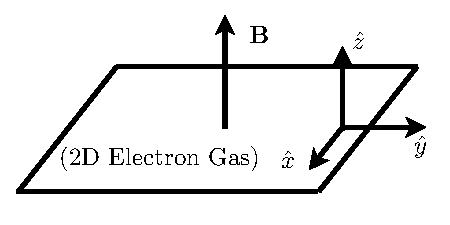
\includegraphics{2dGas.pdf}
		\caption{2D Gas of Non-Interacting Electrons}
		\label{2dGas}
	\end{figure} We will work in the Landau gauge, where $A_x=-B_y$ and $A_y=0=A_z$. Then we have a Hamiltonian
	$$\hat{H}=\frac{1}{2m}\left(\mathbf{p}-\frac{e\mathbf{A}}{c}\right)^2$$
	or
	$$\hat{H}=\frac{1}{2m}\left(p_x-\frac{eB_y}{c}\right)^2+\frac{p_y^2}{2m}$$
	Since this Hamiltonian is independent of $x$, we write the wave function of the electron as
	$$\psi(x,y)=e^{ik_xx}\phi(y)$$
	where $\hat{H}\psi=E\psi$. Then employing Schr\"odinger's equation,
	$$\left(-\frac{\hbar^2}{2m}\partial_y^2+\frac{1}{2}m\omega_c^2(y-y_0)^2\right)\phi(y)=E\phi(y)$$
	where the cyclotron frequency, $\omega_c$ is defined as $\omega_c\equiv \frac{eB}{mc}$, and the equilibrium value of $y$ is $y_0\equiv k_x\ell^2$, where we have introduced the magnetic length,
	$$\ell=\sqrt{\frac{\hbar c}{eB}}=\sqrt{\frac{\hbar}{m\omega_c}}$$
	For perspective, $\hbar\omega_c$ in a 1 Tesla field is equivalent to $1\ \mathrm{K}$, $\ell$ is about 200 \AA.
	
	\subsubsection{Landau Levels}
 	Allowed energies must follow the form of the harmonic oscillators:
	$$E_n=\hbar\omega_c\left(n+\frac{1}{2}\right)$$
	since the Hamiltonian is identical to the quantum harmonic oscillator (a nice product of gauge choice), which then gives energy eigenfunctions
	$$\psi_n=e^{ik_xx}e^{-(y-y_0)^2/\ell^2}H_n\left(\frac{y-y_0}{\ell}\right)$$
	Of interest are the Landau levels, which are highly degenerate, as shown in Figure \ref{landauLevels}. This is because the Hamiltonian does not depend on $k_x$, allowing large number of available states to have the same energy (Check out \emph{Wikipedia}'s entry on Landau Levels!).
	\begin{figure}[h]
		\centering
		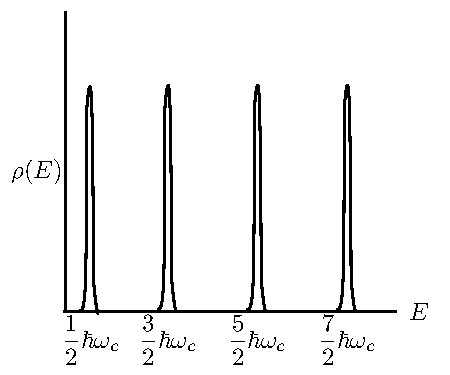
\includegraphics{landauLevels.pdf}
		\caption{Density of States of the Landau Levels}
		\label{landauLevels}
	\end{figure}
	If we confine the system to a box of dimensions $L_x$ and $L_y$, the number of wave numbers $k_x$ is limited to $k_x=\frac{2\pi n}{l_x}$ for some integer $n$. This is from the boundary condition that mandates $\exp(ik_xL_x)=\exp(ik_x0)=1$. This quantization of the wave number necessarily quantizes $y_0$ as well, as
	$$y_0=k_x\ell^2=\frac{2\pi n}{L_x}\ell^2 \Rightarrow \Delta y=\frac{2\pi}{L_x}\ell^2$$
	Thus the available states for each Landau level have the form $e^{ik_xx}$ in the $x$ direction but must necessarily be separated by some multiple of $\Delta y$, as is reflected in Figure \ref{landauDegeneracy}. Since any of these states are accessible, the total number of states is then given by the ratio of $L_y$ and $\Delta y$ (since the state must necessarily be \emph{in} the box)
	$$N_{LL}=\frac{L_y}{\Delta y}=\frac{L_xL_y}{2\pi\ell^2}$$
	\begin{figure}[h]
	\centering
		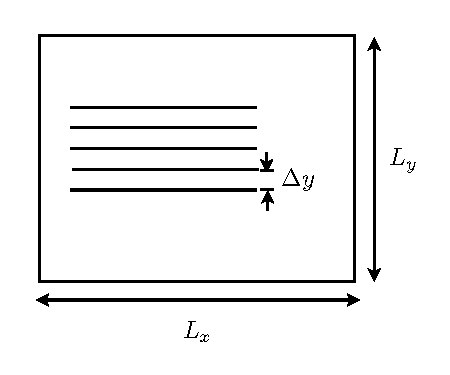
\includegraphics{landauDegeneracy.pdf}
		\caption{Spacing of the Degenerate Landau Level States}
		\label{landauDegeneracy}
	\end{figure}
	For the number density, we want
	$$n_{LL}=\frac{N_{LL}}{L_xL_y}=\frac{1}{2\pi\ell^2}=\frac{B}{\Phi_0}$$
	where $\Phi_0=hc/e$ is the flux quantum. The flux quantum is defined as the amount of flux required for an electron to pick up a phase factor of $2\pi$ while orbiting around the flux. Then we have
	$$N_{LL}=\frac{BL_xL_y}{\Phi_0}=\frac{\textrm{total flux}}{\textrm{quantum of flux}}$$ 
	We define the \textbf{filling factor} $\nu$ to be 
	$$\nu\equiv \frac{N}{N_{LL}}=\frac{\textrm{\#}e^{-}}{\textrm{\# vertices}}$$
	In the integer quantum hall effect, $\nu$ is an integer, and in the fractional quantum hall effect, $\nu=p/q$ for any integer $p$ and any odd integer $q$.
	Suppose we have just enough electrons to fill the lowest Landau Level. Then we have
	$$R_H=\frac{B}{nec}$$
	replacing $n$ with $n_{LL}$, we have 
	$$R_H^{LL}=\frac{B}{n_{LL}ec}=\frac{B}{\frac{B}{\Phi_0}ec}=\frac{h}{e^2}$$
	\subsubsection{Edge Effects in the Integer Quantum Hall Effect}
	Suppose we have a particle in a box in with a confining potential $V(y)$ that keeps the particle from escaping the box. Then the Hamiltonian goes to
	$$\hat{H}\to\hat{H}+V(y)$$
	The wavefunction is still
	$$\psi=e^{ik_xx}\phi(y)$$
	and it now satisfies
	$$\left(-\frac{\hbar^2}{2m}\partial_y^2+\frac{1}{2}m\omega_c^2(y-y_0)^2+V(y)\right)\phi(y)=E\phi(y)$$
	If we assume that $V(y)$ varies slowly near $y_0$ on the scale of $\ell$, we may approximate the confining potential as
	$$V(y)=V(y_0)+V'(y_0)(y-y_0)+\cdots\approx V(y_0)$$
	then the energy levels are shifted
	$$E_n=\hbar\omega_c\left(n+\frac{1}{2}\right)+V(y_0)$$
	Interestingly, these excitations on the edge states are quite similar to one-dimensional Landauer transport, and it corresponds roughly to electrons ``skipping'' along the edge, resulting in a right-moving current on the top and a left-moving current on the bottom.\\
	
	\noindent \textit{April 8, 2011}\\
	
	\noindent Excitations move with a group velocity $v_g=\frac{1}{\hbar}\frac{\partial E}{\partial k_x}$. Now we look at quantization. Let $\mu_S$ be the chemical potential of the source (on the left), and let $\mu_D$ be the chemical potential of the drain (on the right). They are related by
	$$\mu_S=\mu_D+\delta\mu=\mu_D=eV_H$$
	where $V_H$ is the hall voltage. We may now ask what the responding current will be. Let $\delta n$ be the excess density on the top edge whenever $V_H\neq 0$. Then 
	$$I=ev_g\delta n$$
	If the total number of excess electrons is $\delta N$, then
	$$\delta N=\frac{\delta k_x}{2\pi/L_x}\Rightarrow \delta n=\frac{\delta N}{L_x}=\frac{\delta k_x}{2\pi}$$
	This then gives the current as
	$$I=\frac{e}{\hbar}\frac{\delta E}{\delta k_x}\frac{\delta k_x}{2\pi}=\frac{e^2}{h}V_{H}$$
	And then the hall conductance and resistance is naturally
	$$G_H=\frac{I}{V_H}=\frac{e^2}{h}\Rightarrow R_H=\frac{h}{e^2}$$
	This is much like the result from Landauer transport theory, but with $T=1$, as is mandated by the currents present never backscattering. And so we see that the edge states are giving the quantized Hall conductance. In truth, this treatment doesn't \emph{really} explain the quantized effect we see. To do this, we must take into account impurity scattering within the semi-conductor. This becomes rather involved, so we won't be discussing it.
	
	\subsubsection{Fractional Quantum Hall Effect}
	The fractional quantum hall effect is observed when one partially fills the lowest Landau level with a filling factor $\nu=N/N_{LL}$ (Recall $N$ is the number of electrons and $N_{LL}$ is the number of states at that energy). There is a massive degeneracy of many-body states since the electrons in the system can be arranged in any number of combinations of available lowest Landau level states. That is, there are $N_{LL}\ C\ N\sim e^{\alpha N}$ (``$N_{LL}$ choose $N$'') combinations.
	\paragraph{Coulomb Interactions} Interactions between the electrons must now be taken into effect to explain the fractional quantum hall effect. The relevant Hamiltonian, including these interactions, is
	$$\hat{\mathscr{H}}=\sum_{j=1}^N\left[\frac{\mathbf{p}_j-e\mathbf{A}(\mathbf{r}_j)}{2m}\right]^2+\sum_{i<j=1}^N\frac{e^2}{\left|\mathbf{r}_i-\mathbf{r}_j\right|}$$
	Solving this Hamiltonian becomes quite difficult, even using computers due to the exponential growth of the Hilbert space with increasing particle number. In 1993, Bob Laughlin came up with an ingenious solution to the problem: a many-body wave function.
	
	\paragraph{Non-Interacting Electrons in the Radial Gauge} We have been working in the Landau gauge ($\mathbf{A}=yB\,\hat{x}$), whereas Bob Laughlin thought to use the radial gauge, where $\mathbf{A}=\frac{B}{2}\left(x\,\hat{y}-y\,\hat{x}\right)$. For non-interacting electrons in the radial gauge, we follow a similar prescription as the integer quantum hall effect:
	$$\hat{\mathscr{H}}\phi=E\phi$$
	The lowest Landau level is
	$$E_0=\frac{\hbar\omega_c}{2}$$
	and the eigenfunctions are
	$$\phi_n(z)=z^ne^{-\left|z\right|^2/4\ell^2}$$
	where $z=x+iy$ and $n=0,1,2,\ldots$. If we write $z=\left|z\right|e^{i\theta}$, we have $z^n=\left|z\right|^ne^{in\theta}$. Again, the magnetic length is $\ell=\Phi_0/2\pi B$. Let's look into finding the probability of measuring the electron at a position $z$:
	$$\left|\phi_n(z)\right|^2=r^{2n}e^{-r^2/2\ell^2}$$
	This gives a very distribution that is sharply peaked about some $r^*$.
	$$\left|\phi_n(z)\right|^2=r^{2n}e^{-r^2/2\ell^2}=e^{2n\ln r-r^2/2\ell^2}=e^{-f(r)}$$
	$$f'(r^*)=\frac{2n}{r^*}-\frac{r^*}{\ell^2}=0$$
	$$r^*=\sqrt{2n\ell^2}$$
	\paragraph{The Many-Body Wave Function} Now the many-body wave function is
	$$\psi_{LLL}(z_1,\cdots,z_N)=\det A$$
	where $A_{ij}=\phi_{i-1}(z_j)$. Consider $N=2$
	$$\psi_{LLL}(z_1,z_2)=\det\begin{pmatrix}
	1& z_1\\
	1 & z_2\end{pmatrix}e^{-}=(z_2-z_1)e^{-}$$
	For $N$ particles, the solution is
	$$\psi_{LLL}(z_1,\cdots,z_N)=\prod_{i<j=1}^N(z_i-z_j)e^{-\sum_{j=1}^N\left|z_j\right|^2/4\ell^2}$$
	This function is anti-symmetrized, as required, but not quite right. Bob Laughlin won his Nobel prize for making one small change: a 3 in the exponent of the $z_i-z_j$ term to represent the 1/3 filling factor state:
	$$\psi_{LLL}(z_1,\cdots,z_N)=\prod_{i<j=1}^N(z_i-z_j)^me^{-\sum_{j=1}^N\left|z_j\right|^2/4\ell^2}$$
	This must necessarily be an odd integer to keep the wave function anti-symmetrized.
	\paragraph{Electron Density}	
	$$\prod_{i<j=1}^N(z_i-z_j)^m\longrightarrow z_1^{m(N-1)}$$
	This is the maximum power of $z_1$, giving it the the largest possible angular momentum.
	$$\frac{R}{\ell}=\sqrt{2m(N-1)}$$
	The actual density of the electrons in the disk is
	$$n=\frac{N}{\pi R^2}=\frac{1}{2\pi\ell^2m}$$
	This mandates the filling factor be
	$$\nu=\frac{N}{N_{LLL}}=\frac{n\pi R^2}{(B\pi R^2)/\Phi_0}=\frac{hc}{e}\frac{n}{B}=n(2\pi\ell^2)=\frac{1}{m}$$
	We do, indeed, observe the fractional quantum hall effect with filling factors of $1,1/3,1/5,1/7,\ldots$.
\end{document}